\subsection{Creating Questions}
%Todo update media part if any changes have been done, fix the images.
Everything in the application that is restricted to admin will only use the admin.vue component as the view file. In order to start creating questions you’ll have to load the Question.vue component onto the admin.vue view. You do this by clicking on the Questions tab on the dashboard, this will call a method in Admin.vue that will you use the vue router to update the path to /admin/questions which will make the admin.vue load the needed Question.vue component. The Question.vue component consist of other components such as EditQuestion.vue, ShowQuestion.vue, SelectCourse.vue and AddQuestionToSession.vue. All components that is related to creating a question can be found in the App/client/components/admin/question folder. On the /admin/question page there will be a select form to the left, which is the SelectCourse component. In this select form the user can choose between the available courses in the database. Keep in mind that a course must be chosen for the user to able to create new question. This is done so that a question will immediately be assigned to the given course, since every question should to be assigned to at least a single course before the question should allowed to be used in an active session.  If the user tries to create a question without there being a course in the database, an error message will be displayed instead.\\[11pt]
The area with white background is where the current questions for the selected course will be listed. If there are no questions for the given course, then a message “no question” will be displayed instead. Whenever the Question component is loaded, the course is changed, a question is edited or created, a socket emit request is sent to the server. This emit message will ask server for all the current questions for the current selected course. The server then calls the appropriate select statement in the database and returns the result. The result is then used by the Question component to update the list of questions. In this way the list should be always up to date with the contents in the database. 
\begin{figure}[H]
	\centering
	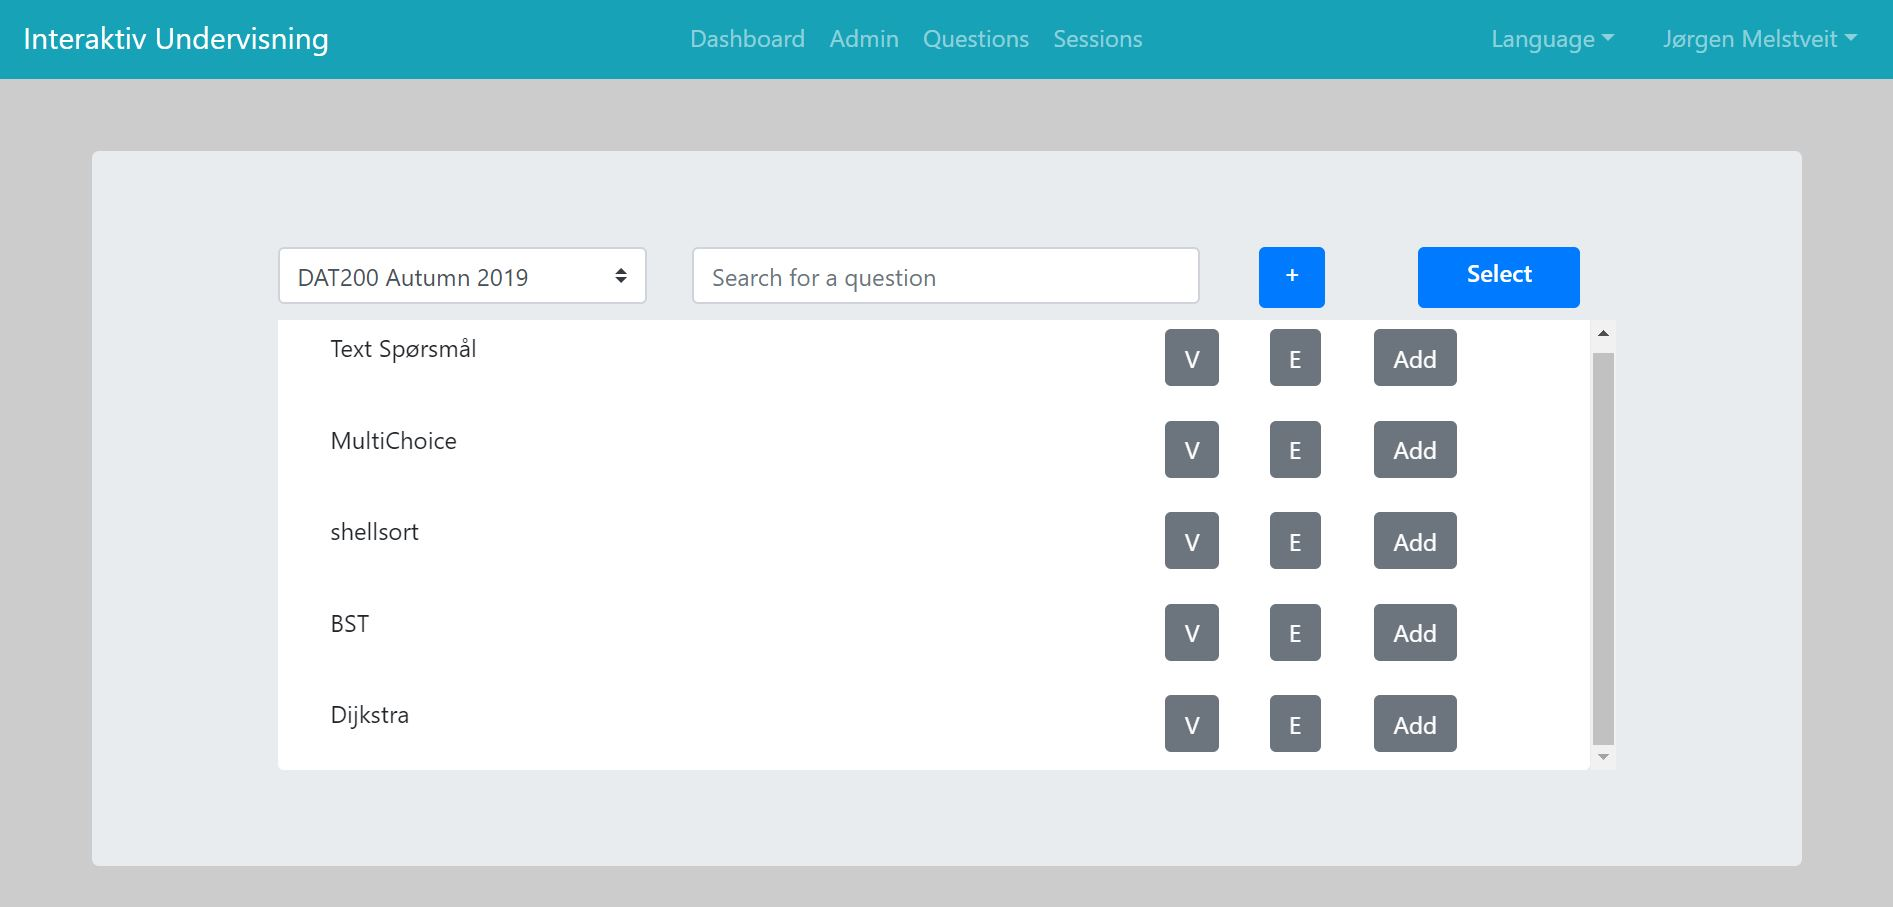
\includegraphics[width=0.80\linewidth]{/createQuestion/questionvueEnglish}
	\caption{The figure displays an image of the Question.vue. This is the component is primarly used for allowing users to create new questions for a selected course. It uses the vue path /admin/questions}
	\label{fig:questionVue}
\end{figure}
To create a new question all the user needs to do is to click on the button with the label “+”. This will show the EditQuestion component which contain a vue modal element that has all the needed forms needed for creating a question. There may be some confusion revolving the name of the EditQuestion component since it called edit when the component is used for adding new questions. EditQuestion is a component that is used for both adding new questions and editing existing questions. The main difference between the add and edit operation for the component is that title of the modal will be different, edit will have to load the data from the database and fill in the forms accordingly and finally the request sent to the server once the ok button is clicked. The server request is different primarily to distinguish between the insert and update command needed for the database. Originally there were 2 components used for the two operations, but this was later changed in development because having 2 components that were practically was deemed unnecessary. The modal is divided into 3 parts, namely Basic Information, Media and Solution type.  These parts can be opened and closed to the users preference, where basic information will be opened by default and the other parts will be closed. Though a user needs to fill inn at least the information in basic information and solution type in order for the wanted question to be valid. Basic Information part contains an input field for assigning the question title, a textbox for giving the question a description, a time input field and a time slider. The input for title, the textbox and the time slider are all using v model to mount to a variable in the data layer so that data in these fields are relatively easy to acquire and keep track of. The time input has a watcher that checks for changes to the variable that the time slider is mounted to. This means in that these elements always changing their value dependent on the other, resulting in them having the same value. If the time is set to “00:00”, then the question will not have a timer when used in a session.\\[11pt]
The media part is an optional part and is not required to be used to make a new question. By clicking on the “Media” label the EditQuestion component will show a select box and button. The select box is used for choosing the wanted media type. The button is for adding an image to the question. By clicking on the button, a file browser will be displayed for the user and allow them to choose an image on their computer and put it onto the question. Once the image is chosen, the EditQuestion component will take the image and then validate the image given, in order to be sure that the file taken was an actual image file. If the validation passes, then the image is turned into a buffer. When the question is going to be saved on the database, the question will also contain the file paths to the images given to the question. The buffer is then sent to the server and is turned back into an image and is stored in on the path stored in the database. Whenever a question is obtained from the database that has images, the server will collect the images will by using the routes stored with the question. When the image is going to be used on the client again the image will be transformed back into a buffer. A question cannot have to many images assigned to it, as this would take up a lot of the needed data. The total amount of files attached to a question cannot exceed 1.5MB, and the user will get a warning once the amount exceeds 500KB.\\[11pt]
The solution type part focuses on setting the type of question the new question is going to be and creating the solution for the question. The type will control what format the question will have for both the solution and for the client during a session. Most of the question types available are usually centred around a data structures or an algorithm. There exist also normal question types like multichoice and text questions. The question type chosen will alter the available options in the solution type, so that the user can fill in the information needed for certain algorithm. For instance, Binary Search, AVL and Dijkstra question types all require the GraphDrawer tool. The solution for questions revolving data structures and algorithms are created on the server. The user only needs to apply the necessary information for the question so that its possible for the student to solve it and for the server to be able to create a solution. As stated, before the necessary information needed for the question is determined by the question type. The reasons for having the server handling the solution is that the solution should not be easily accessible to the clients participating in a session, but also because making the user write the entire solution for an algorithm in every question created would be rather tedious for the user. Not to mention reducing the chances of having the solution being incorrect.
%TODO merge all the EditQuestion opened images into a single image, and then display it together with the unopened one. Update the caption and labels accordingly.
\begin{figure}[H]
	\centering
	\begin{subfigure}{0.30\linewidth}
		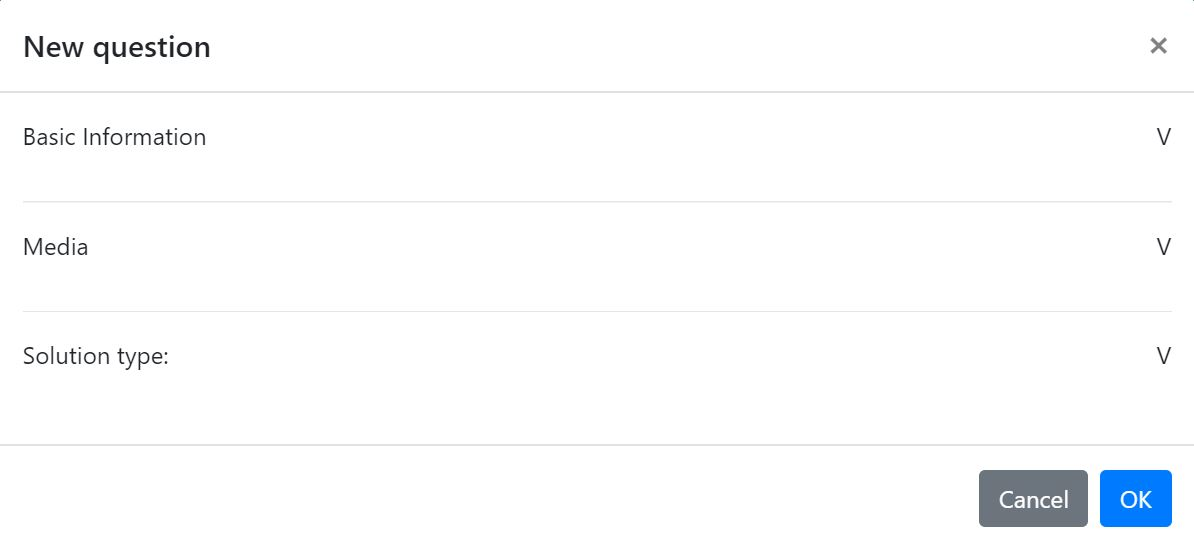
\includegraphics[width=\linewidth]{/createQuestion/editQuestionUnOpenedEnglish}
		\caption{This figure displays an image of the editquestion component when all the 3 parts Basic Information, Media and Solution type are hidden. Click on the labels would reveal the content of chosen part.}
		\label{fig:editquestionUnOpened}
	\end{subfigure}
\end{figure}
Once the question is finished the user only needs to click the button labelled ok to send the information to the server. The data sent to the server is the newQuestion object found in the function initializeState() in the EditQuestion component. Since all the variables in the newQuestion object are linked to the vue component, the server should have all the information needed to create the solution and store it in the database together with the question information. However, to avoid any problems regarding storing faulty questions on the server, the question information will first need to be validated by the server's validation checker. The question information sent to the sever will first be validated on the basic information in the question, then another validation test that is determined by the given questions type.  If validation checker returns false, then the question failed the validation criteria and the error given by the validation checker will be returned on the EditQuestion component as an alert box. If the validation succeeds, then the information is sent to the solution generator that generates the appropriate solution in accordance to the questions type. Once this is done, the question information and solution are inserted into the question table in the database. In parallel to this the EditQuestion component will be closed and the user will return to the Question component. The Question component will then update its question list to accommodate for the changes just done on the database.
\\[11pt]
Once a question is created and is listed on the Question component, there will be more options available for the user regarding the question. First of clicking on the button with the label “E” will open EditQuestion component and let you edit the information previously saved for the question. Do keep in mind that the changes to the existing question aren't going to be saved unless the ok button is pressed and the request is fully validated by the server, just as with the add functionality. It is also not possible to edit a question type once it’s been assigned to a session. \\[11pt]
Next by clicking on the button labelled “V” the component ShowQuestion will be visible. This component will load in all the information regarding the question where the V button the user clicked belonged. The ShowQuestion consist of a v modal that has similar design to the EditQuestion component. Its divided into the same three parts as the EditQuestion, where Media is only shown in the component if any images where included in the question. By clicking on basic information label, the user can view the basic information of the question like title, description and the time limit. By clicking on media label, the user can view all the images currently linked to the question. This includes information about the file such as name, type and the size. Finally, by clicking on the solution label the solution for the question will be displayed. What is shown is depend on the solution type. Text, multichoice and binary tree will show the answer/answers in plain text, while every other question type will use the GraphDrawer to display the solution. The user can close the component by either clicking on the cross in the top right or by clicking on the button labelled “Close”. 
%TODO merge the opened ShowQuestion images into a single image, then display it together with the unopened one. Update the caption and labels accordingly
\begin{figure}[H]
	\centering
	\begin{subfigure}{0.80\linewidth}
		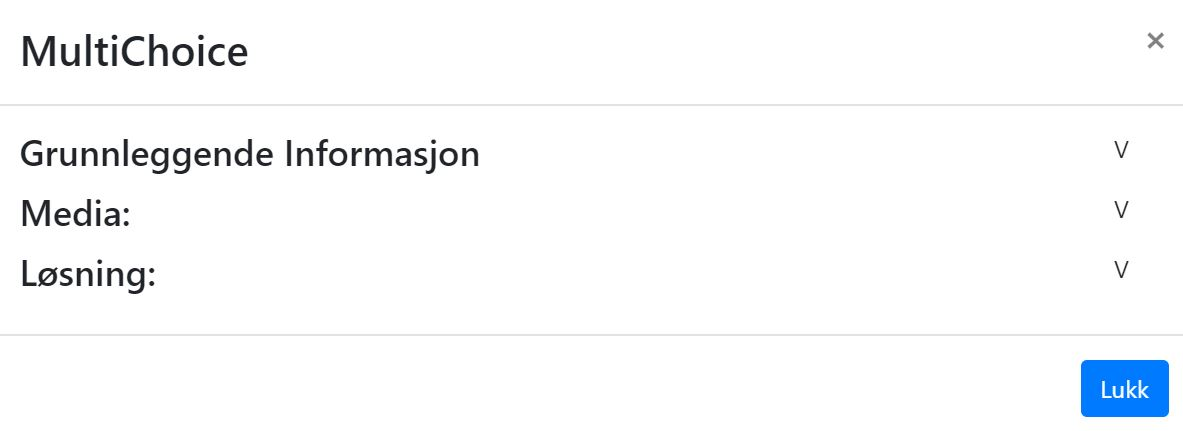
\includegraphics[width=\linewidth]{/createQuestion/showQuestionEnglishUnOpened}
		\caption{This figure displays an image of the ShowQuestion component while all the 3 parts are closed. Clicking on the labels should open op the chosen part.}
		\label{fig:showQuestionUnOpened}
	\end{subfigure}
	\begin{subfigure}{0.32\linewidth}
		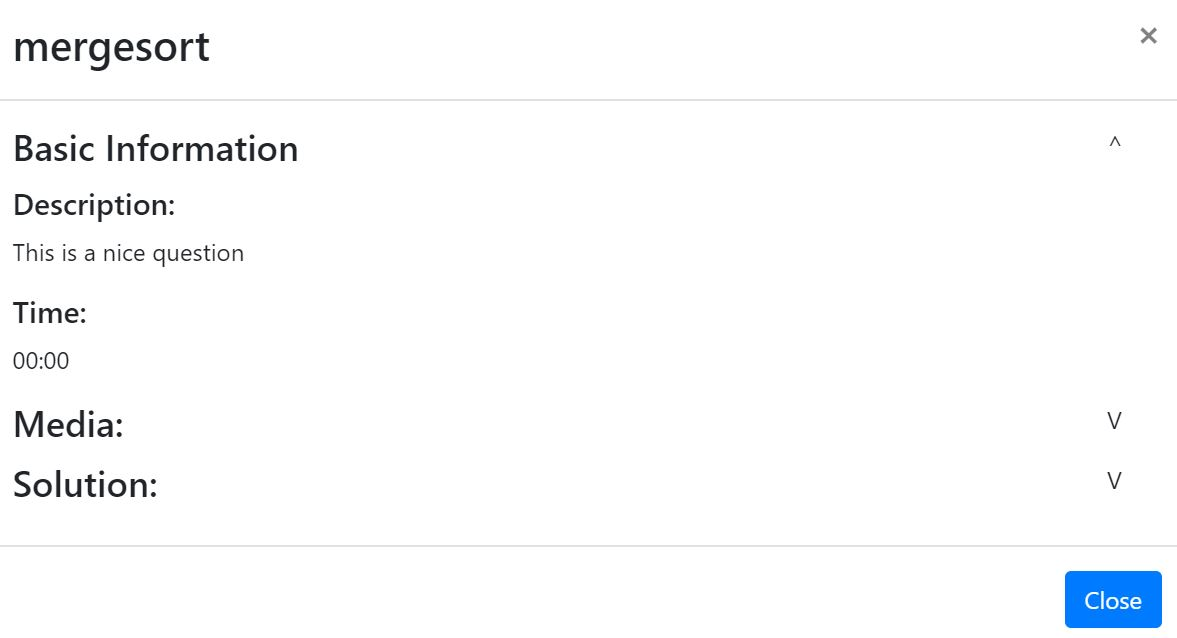
\includegraphics[width=\linewidth]{/createQuestion/showQuestionEnglishBasicOpened}
		\caption{}
		\label{fig:showQuestionBasicOpened}
	\end{subfigure}
	\begin{subfigure}{0.32\linewidth}
		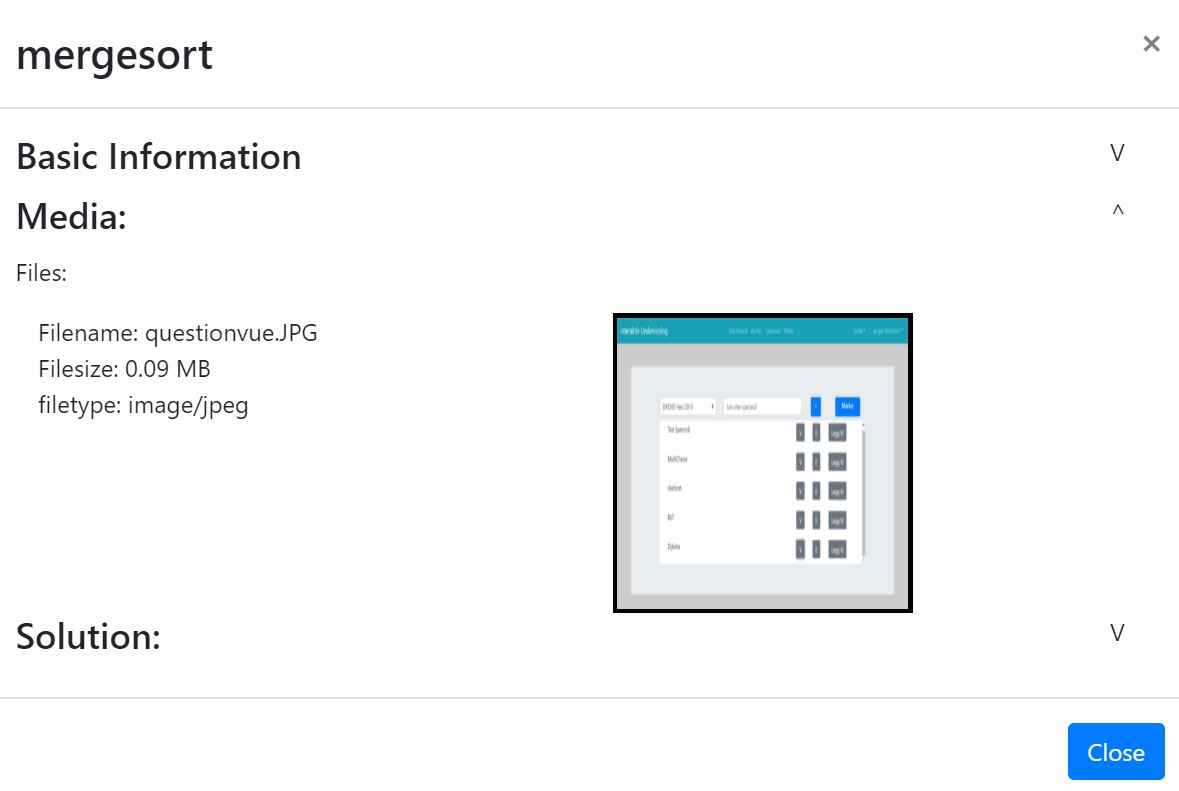
\includegraphics[width=\linewidth]{/createQuestion/showQuestionEnglishMediaOpened}
		\caption{}
		\label{fig:showQuestionMediaOpened}
	\end{subfigure}
	\begin{subfigure}{0.32\linewidth}
		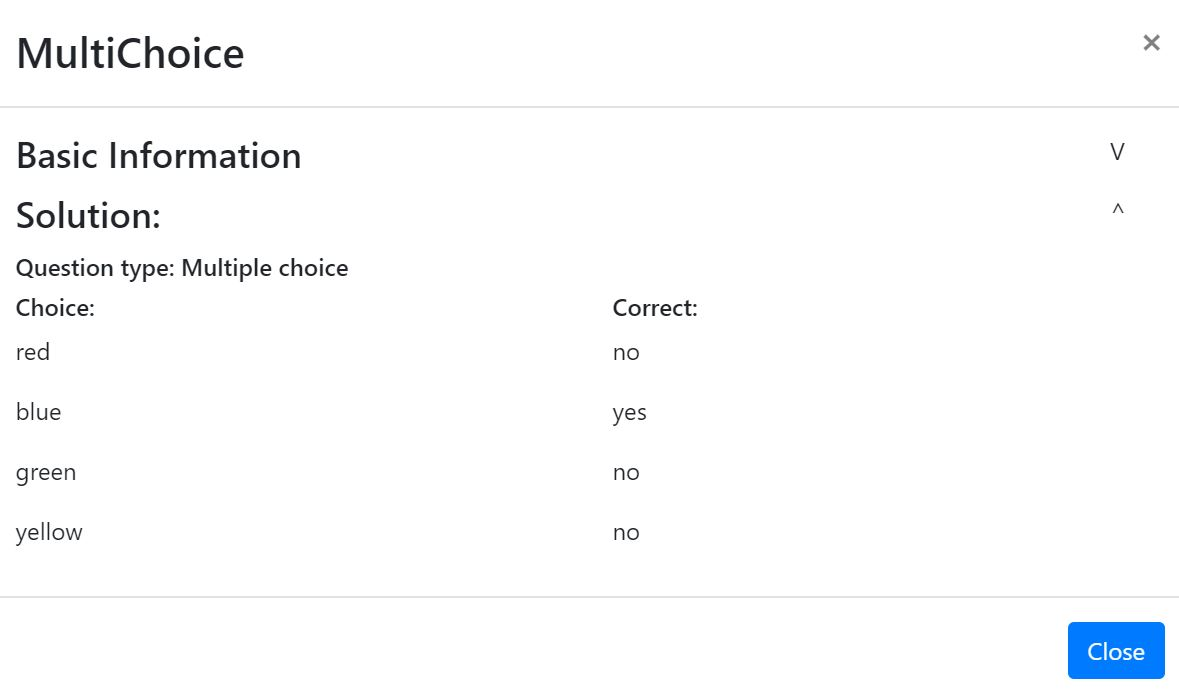
\includegraphics[width=\linewidth]{/createQuestion/showQuestionEnglishSolutionOpened}
		\caption{}
		\label{fig:showQuestionSolutionOpened}
	\end{subfigure}
\end{figure}
The last button labelled Add will show the addQuestionToSession component. This component will only display a select box containing all current available sessions in the database. The user can select one of these sessions and by clicking the button labelled “Ok” the question of which the Add button belonged to will be added to the chosen session. This was implemented to give admins the options of adding more questions to an existing session, without having to create an entirely new session just for adding an extra question.\\[11pt]
Lastly the Question component allows you to mark question in the list by clicking on the button with the label “Select”. Once the button is used, the user has the option of clicking on the list items and either copy the selected questions to another course or deleting the questions from the current course. To copy simply click on the green button labelled “Copy” and to delete the questions simply click on the red button labelled “Delete”. To exit the select mode simply click on the select button again, which now has the label “Close”. The copy button will use the CopyQuestions component while the delete button will use the DeleteQuestions component. If the user tries to click on the copy or remove buttons without having selected a question, then an alert box will appear stating that there are no questions being selected. Keep in mind that its currently not possible to remove questions from a course if its already been used in a session. The reason for this is that the question information is still needed for feide users to look at the previous participated sessions. If the question were to be removed after having been used in a session, then the student wouldn't have access to the question information, neither the students old result. \\[11pt]
The question structure for this application was specifically chosen in a way it would be easier for developers to implement and add new questions types. Excluding the work that is needed for writing the actual data structure or algorithm and its solution format, all that is required in order for a new question type to be added to a session is the following. Create a vue component in both the questionResultScreenAnswer and questionResultScreenSolution. These are going to be used for DisplayQuestion component which is used for showing session results after each question. Next add a b-form-group to the EditQuestion component where only the necessary form items and Graphdrawer are set so that the user can create the new question type. If the question type requires a certain unique information, then an extra variable in the newQuestion.objects in the initializeState function should also be assigned and model appropriately to the html element in the form group. Then add a js file in the validation checker for stopping illegal actions to the new type. Then implement the solution generator for the question type which is going to create the format for the solution object stored in the database. Finally create a solution checker that is going to verify that the student answered correctly according to the solution object that was withdrawn from the database. The user may also have to update the locale files as well if some new predefined text is needed.\\[11pt]

 